\chapter{IPv6-Multicast}
\label{chap:ipv6_multicast}

\section{Ejercicio 3.1}
\subsection{En los primeros 2 segundos de simulación se envían varios paquetes NS. Muestra una captura del tráfico de
paquetes en Wireshark en la que se vean las direcciones IP y MAC origen y destino de los NS enviados desde
cada uno de los nodos host[*]. (Nota: para mostrar las direcciones MAC añade dos nuevas columnas: Hw src
addr (unresolved) y Hw dest addr (unresolved). Colócalas a la derecha de las direcciones IP.) ¿De qué tipo son
las direcciones IP? ¿Cómo se construyen?}

\begin{figure}[H]
    \centering
    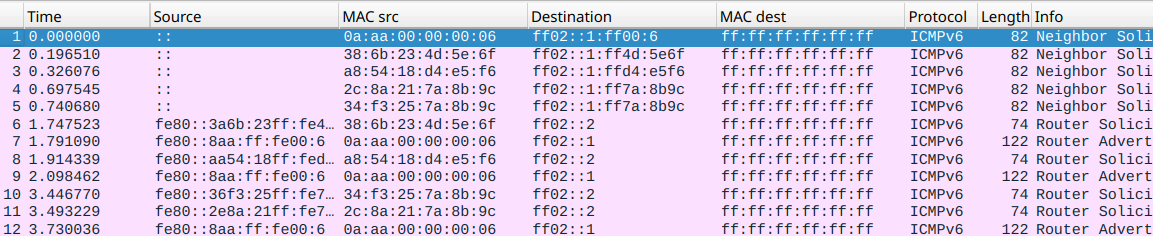
\includegraphics[width=135mm, scale=0.75]{imaxes/captura_ejer3_1.png}
    \caption{Captura MAC origen y destino host[0]}
    \label{fig:ip_mac_host0}
\end{figure}

Como las direcciones IPs de destino son multicast, en todos los hosts se ve la misma paquetería, por lo que solo subimos la captura de tráfico en el host[0].

Las direcciones, como hemos mencionado anteriormente, son multicast y se construyen con el prefijo multicast link-local (FF02::1, donde FF02 quiere decir que es tipo multicast, siendo el 2 un scope de local de enlace y el último 1 quiere decir todos los dispositivos. Si fuera un 2 serían todos los routers). Por último, tendríamos como sufijo, los 3 bytes menos significativos de la MAC del dispositivo de ese host precedido de FF.

Por ejemplo, en el primer caso tenemos como destino FF02::1:FF00:0006 donde F002::1 es, como explicamos antes, el prefijo multicast link-local y como sufijo FF00:0006, donde 000006 son los 3 últimos bytes de la MAC de la interfaz del router en ese enlace (0A:AA:00:00:00:06).

\section{Ejercicio 3.2}
\subsection{¿Coincide alguna de las direcciones IP destino de los diferentes paquetes NS? ¿Por qué? ¿Qué consecuencia
tiene esto?}

Coinciden las direcciones IP del host[0] y host[2], ya que los dos tienen los 3 últimos bytes de la MAC iguales por lo que la dirección multicast se construye de la misma forma.

Con respecto a las consecuencias que se puede tener al haber dos direcciones multicast iguales, no hay ninguna, ya que los mensajes ICMPv6 de tipo NS (Neighbor Solicitation) guardan en su cabecera la dirección unicast de destino, por lo que no se daría ningún conflicto (target address). Aunque no pase nada, lo normal es que las direcciones multicast de nodo solicitado (FF02::1) sean únicas.


\section{Ejercicio 3.3}
\subsection{¿Por qué se envían los NS a esas direcciones IP?}

Se envían ICMPv6 de tipo NS a esas direcciones ya que haciéndolo con direcciones multicast, se puede mandar un único paquete a uno o varios destinos, de esta forma optimizamos la comunicación y reducimos el tráfico de la red para que no se congestione por lo que aumenta la eficiencia. 


\section{Ejercicio 3.4}
\subsection{¿Qué direcciones MAC destino tienen los paquetes NS anteriores? ¿Cuáles deberían tener según lo visto en
clases de teoría? (Utiliza el paquete NS que sale desde host[1] como ejemplo y escribe los 6 bytes que debería
tener la dirección MAC en formato hexadecimal.)}

\begin{figure}[H]
    \centering
    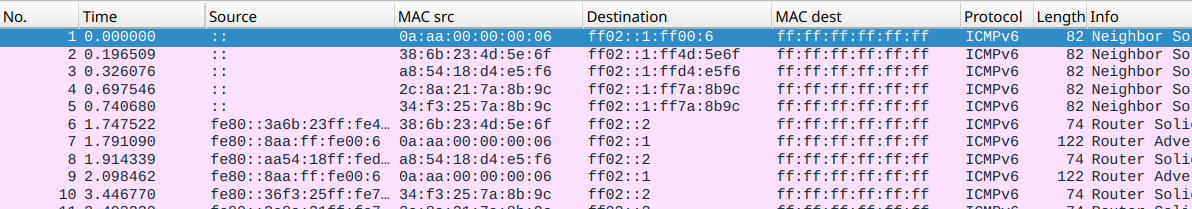
\includegraphics[width=135mm, scale=0.75]{imaxes/captura_ejer3_4.png}
    \caption{Captura MAC origen y destino paquetes NS en host[1]}
    \label{fig:ip_mac_host1}
\end{figure}

Como se puede observar en la imagen \ref{fig:ip_mac_host1}, todos los paquetes tienen como MAC destino FF:FF:FF:FF:FF:FF. Según se ha visto en la clase de teoría, las MAC tienen la estructura 33:33:FF como prefijo de la MAC y, después, los 3 últimos bytes son los 3 bytes menos significativos de la dirección multicast. En este caso, el destino es la dirección MAC broadcast, ya que Omnett no sabe como construir este tipo de direcciones MAC como se explica en la teoría, por eso todos los hosts reciben la misma paquetería. De la otra forma, cada uno recibiría su propia paquetería.

\section{Ejercicio 3.5}
\subsection{¿Qué consecuencia tiene esta diferencia con respecto a lo visto en clase de teoría?}

Resulta que las consecuencias de usar dirección MAC broadcast es que todo el mundo recibe paquetes que en realidad no tendrian que recibir por lo que se sobrecarga la red. Usando la direccion MAC que se especifica en la teoria, solamente se mandaría el paquete a ese host.

\section{Ejercicio 3.6} 
\subsection{Muestra las direcciones IP y MAC destino de los mensajes RS y RA que aparecen en torno al segundo 2 de
simulación. ¿De qué tipo son las direcciones IP?}

\begin{figure}[H]
    \centering
    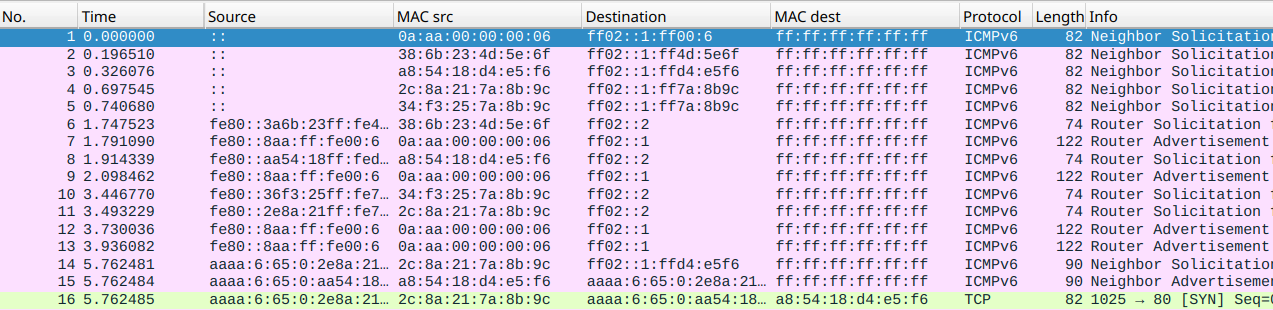
\includegraphics[width=135mm, scale=0.75]{imaxes/captura_ejer3_6.png}
    \caption{Captura paquetes RS y RA host[0]}
    \label{fig:rs_ra_h1}
\end{figure}

Como se puede observar en la imagen \ref{fig:rs_ra_h1}, en el caso de los paquetes ICPMv6 con mensaje RS tienen como dirección destino la direccion multicast FF02::2 y como MAC de destino, la dirección FF:FF:FF:FF:FF:FF. En este caso, las direcciones multicast son de este tipo ya que son direcciones a las que van dirigidos los paquetes a todos los routers de la misma red de en enlace para así optimizar el proceso de descubrimiento de routers y no malgastar ancho de banda.

En el caso de los paquetes ICMPv6 con mensaje RA, estos tienen como dirección destino la dirección multicast FF02::1 y como MAC de destino la dirección FF:FF:FF:FF:FF:FF. En este caso, la dirección multicast tiene esta estructra ya que va dirigido a todo dispositivo que está en el mismo enlace de red. 

\section{Ejercicio 3.7}
\subsection{¿Por qué el RA de respuesta a un RS no usa IP destino unicast?}

Este enfoque permite enviar la información de configuración a todos los dispositivos de la red sin necesidad de identificar la dirección específica de cada uno. Si se utilizara una dirección unicast, sería necesario conocer la dirección única de cada dispositivo, lo que resultaría poco práctico en redes grandes o cuando los dispositivos conectados pueden cambiar con frecuencia. Así, de esta forma, el tráfico no se sobrecarga y resultaría todo mas eficiente.

\section{Ejercicio 3.8}
\subsection{¿Qué direcciones MAC destino deberían tener los RS según lo visto en clases de teoría? ¿Y los RA?}

La MAC destino del paquete RS debería ser 33:33:00:00:00:02, asegurando que solo los routers reciban las solicitudes de descubrimiento de nodos, y los paquetes RA deberían tener como MAC destino 33:33:00:00:00:01, por lo que así sería captado por las interfaces Ethernet de todos los dispositivos IPv6 de esa misma red.

\section{Ejercicio 3.9}
\subsection{ Aproximadamente en t = 6 s el router envía dos NS. ¿De qué tipo son las direcciones IP destino de estos
paquetes? Explica cómo se construyen (notación IPv6 no abreviada).}

En IPv6, las direcciones de destino de los mensajes de Neighbor Solicitation son direcciones multicast de nodo solicitado. Estas direcciones se utilizan en el protocolo Neighbor Discovery para resolver la dirección MAC correspondiente a una dirección IPv6 de destino específica en la red local o para anunciar la presencia del emisor del paquete en el proceso de Duplicate Address Detection (El caso estudiado en este ejercicio es el especificado en primer lugar). Cada dirección unicast IPv6 tiene asociada una dirección multicast de nodo solicitado, las cuales, a su vez, se corresponden siempre con una direccion multicast Ethernet.\\
Las direcciones multicast de nodo solicitado se forman añadiendo tras el prefijo \\
FF02::1:FF00:0000/104 (ff02:0000:0000:0000:0000:0001:ffXX:XXXX) los 24 bits menos significativos de la dirección unicast correspondiente. \\
En nuestro caso, como se observa en el paquete 15 de la figura \ref{fig:ns_from_router_to_host0}, la dirección de destino es, siguiendo la notacioón IPv6 no abreviada, 
ff02:0000:0000:0000:0000:0001:ff7a:8b9c. De esta forma, el paquete será procesado solo por aquellos equipos cuya dirección unicast termine por 7a:8b9c, aunque sea enviado a todos los nodos en la red del destinatario.

\begin{figure}[H]
    \centering
    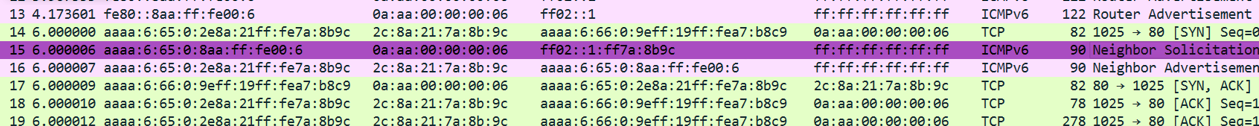
\includegraphics[width=135mm, scale=0.75]{imaxes/ejercicio3_9_1.png}
    \caption{Intercambio de paquetes en t=6 entre el router y host[0]}
    \label{fig:ns_from_router_to_host0}
\end{figure}

\section{Ejercicio 3.10}
\subsection{¿En qué equipos llega el segundo paquete NS enviado por el router al módulo ipv6? ¿Y al submódulo
ipv6.neighborDiscovery? ¿Por qué? (Nota: para ver el recorrido del paquete en el módulo ipv6, haz doble click en
el nodo deseado y luego en el módulo ipv6. Puedes mostrar varios nodos a la vez en diferentes ventanas con
botón derecho → Open Graphical View for ‘ipv6’ una vez dentro de ese nivel.)}

En primer lugar, cabe destacar que el segundo paquete NS al que nos referiremos en este ejercicio es el que aparece en la figura \ref{fig:ns_from_router_to_host0}, es decir, el enviado del router al switch de la LAN a la que está host[0] conectado. Esto se sabe, porque, como se aprecia en la figura \ref{fig:ns_logs}, el primer paquete (Evento 569) es enviado hacia el servidor remoto; mientras que el evento 605 refleja el envío de ese segundo paquete hacia la dirección multicast de nodo solicitado de host[0].\\
El paquete NS es primero enviado al switch, que, a su vez, lo reenvía a todos los hosts y a server\_local. Esto se debe a que INET no implementa correctamente direcciones MAC multicast, por lo que la dirección de nodo solicitado de destino equivale a la dirección broadcast de capa 2, ff:ff:ff:ff:ff:ff (Ver \ref{fig:ns_from_router_to_host0}). Podemos ver en detalle en las figuras \ref{fig:ns_ipv6_host0} y \ref{fig:ns_ipv6_host1}, que el paquete entra al módulo IPv6, tanto de host[0] como de host[1], que realmente no es el objetivo de esta transmisión (De igual forma ocurre en server\_local y host[2]).\\
Por otra parte, se puede ver en la comparación representada en la figura \ref{fig:ns_ipv6ND_host0host1} entre host[0] y host[1], el paquete solo pasa al módulo neighborDiscovery en el caso de host[0], ya que es previamente procesado en el módulo IPv6, donde sí puede leerse su dirección destino de nodo solicitado. Sin embargo, debido a que host[0] y host[2] tienen los últimos 3 bytes de su MAC, y por lo tanto, de su direccción multicast de nodo solicitado, idénticos, el paquete es recibido también en el módulo IPv6 de host[2] (Ver \ref{fig:ns_ipv6ND_host2}).\\
En resumen, el paquete NS alcanza el módulo IPv6 de host[0], host[1], host[2] y server\_local y el módulo neighborDiscovery de host[0] y host[2], únicamente. 

\begin{figure}[H]
    \centering
    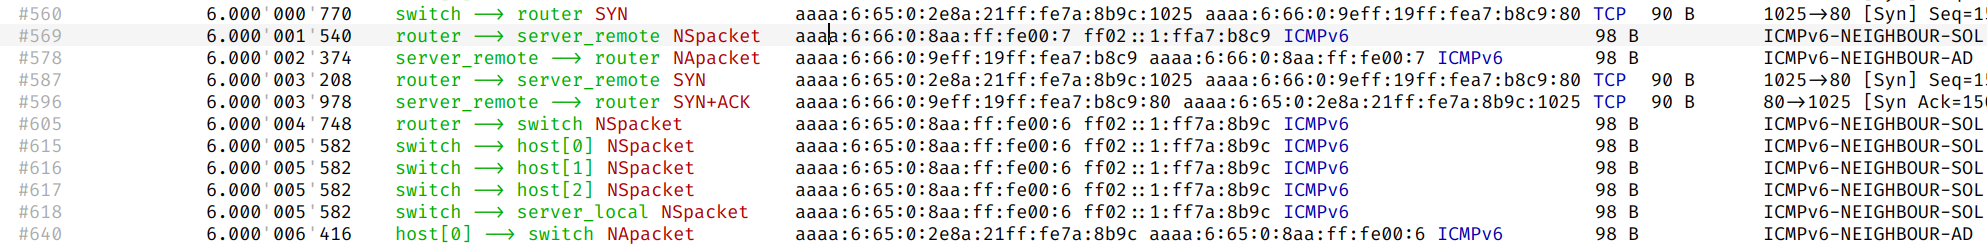
\includegraphics[width=135mm, scale=0.75]{imaxes/ejercicio3_10_1.png}
    \caption{Paquetes enviados por el router en t=6 (Captura de log)}
    \label{fig:ns_logs}
\end{figure}

\begin{figure}[H]
    \centering
    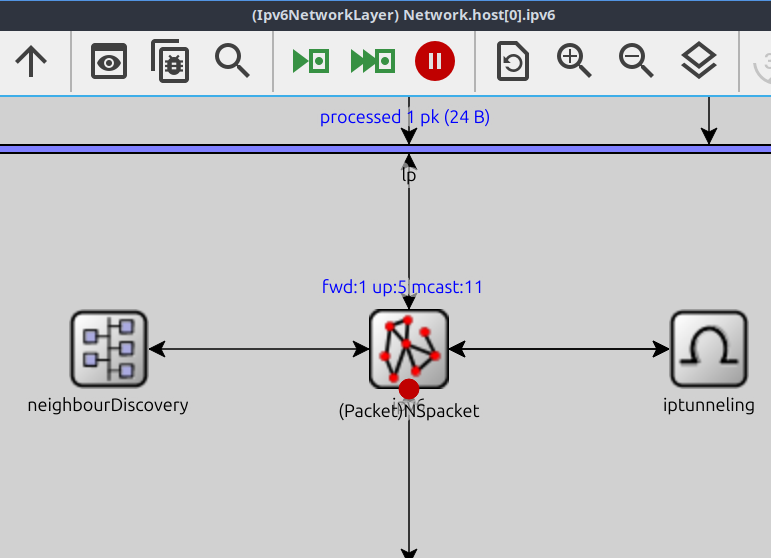
\includegraphics[width=135mm, scale=0.75]{imaxes/ejercicio3_10_2.png}
    \caption{Paquete de NS entrando al módulo IPv6 de host[0]}
    \label{fig:ns_ipv6_host0}
\end{figure}

\begin{figure}[H]
    \centering
    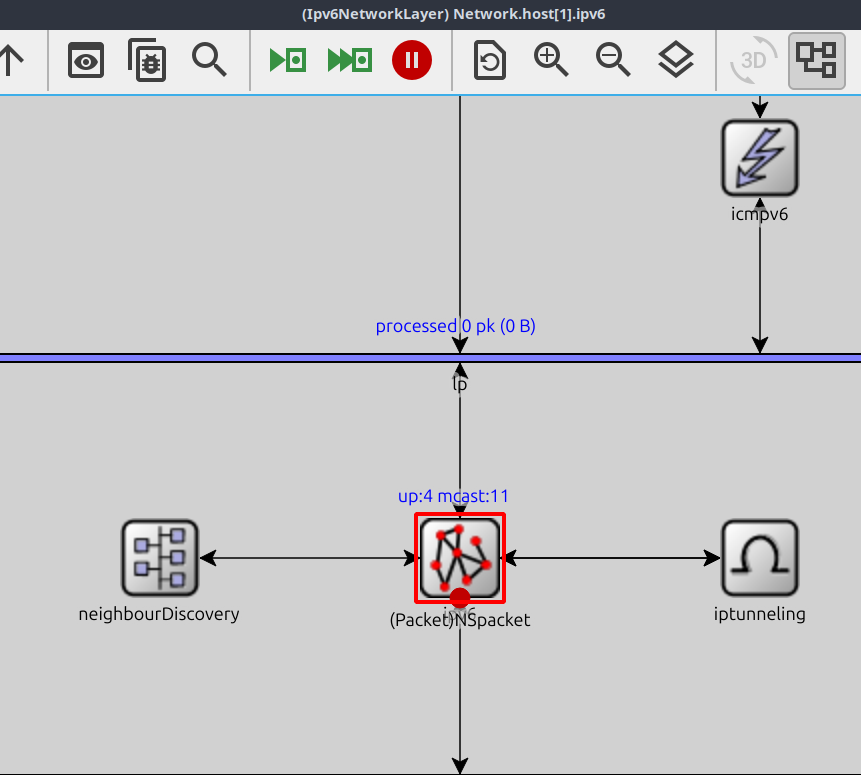
\includegraphics[width=135mm, scale=0.75]{imaxes/ejercicio3_10_3.png}
    \caption{Paquete de NS entrando al módulo IPv6 de host[1]}
    \label{fig:ns_ipv6_host1}
\end{figure}

\begin{figure}[H]
    \centering
    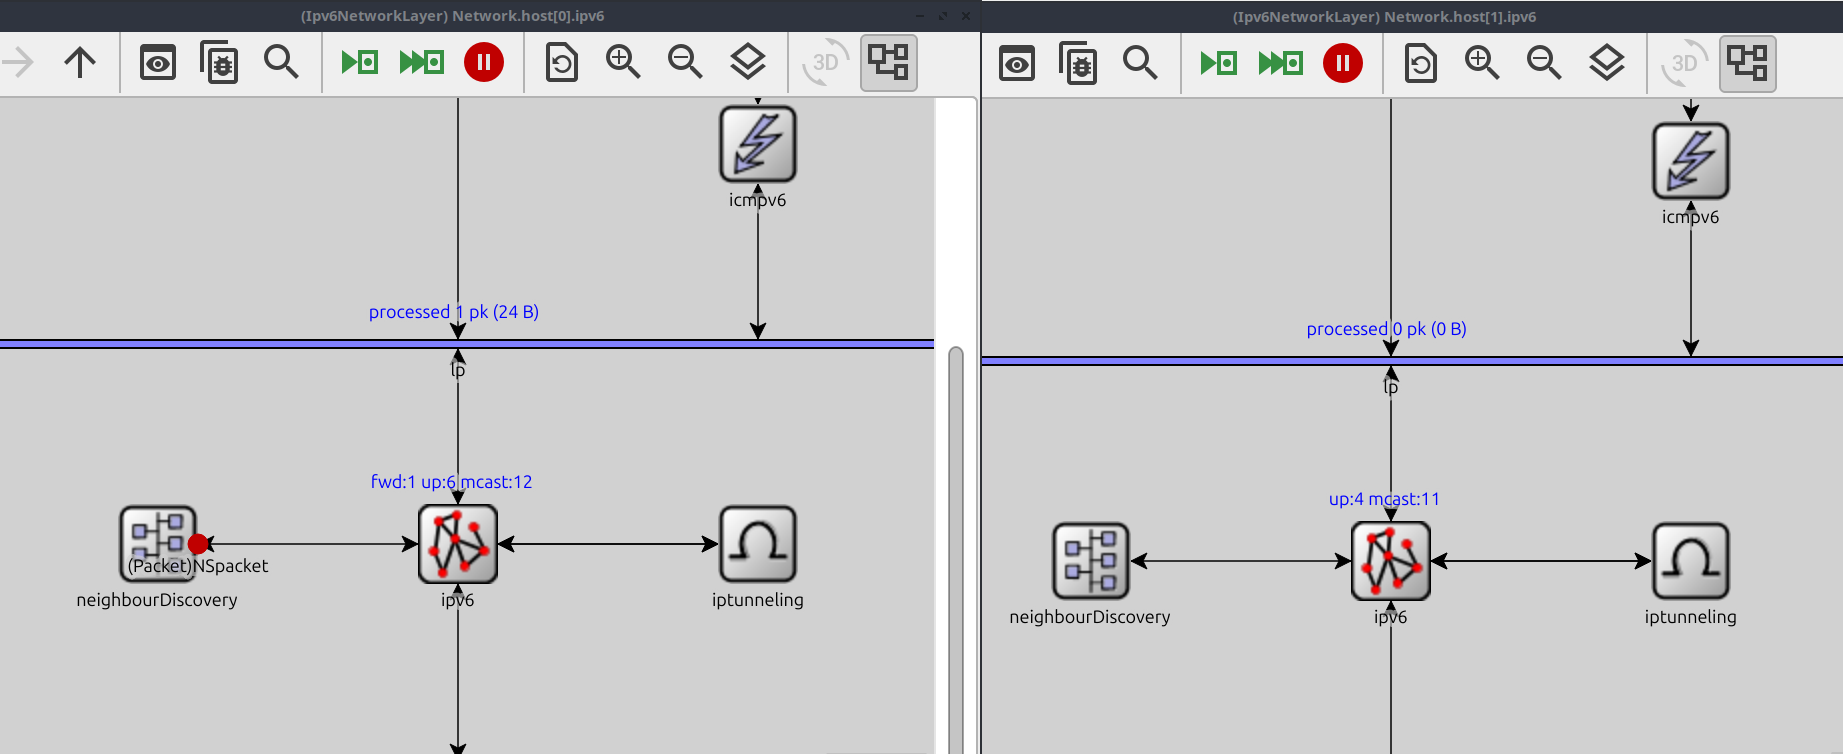
\includegraphics[width=135mm, scale=0.75]{imaxes/ejercicio3_10_4.png}
    \caption{Comparación entre host[0] y host[1] de paquetes entrantes al módulo neighborDiscovery}
    \label{fig:ns_ipv6ND_host0host1}
\end{figure}

\begin{figure}[H]
    \centering
    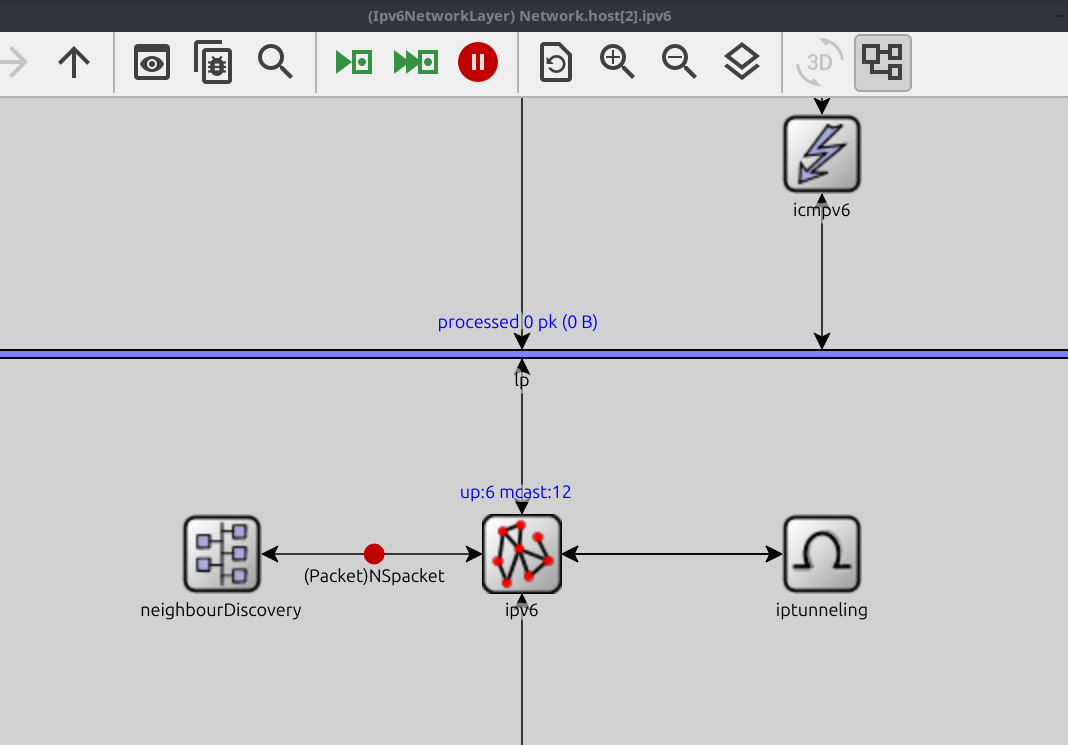
\includegraphics[width=135mm, scale=0.75]{imaxes/ejercicio3_10_5.png}
    \caption{Paquete de NS entrando al módulo neighborDiscovery en host[2]}
    \label{fig:ns_ipv6ND_host2}
\end{figure}

\section{Ejercicio 3.11}
\subsection{¿En qué equipos llegaría el mensaje al módulo ipv6 si INET implementase direcciones MAC multicast (33-
33-xx-xx-xx-xx)? ¿Por qué?}

Si INET implementase este tipo de direcciones, el mensaje llegaría al modulo IPv6 (Prefijo 33-33) de los equipos que tengan asignada la dirección MAC 33-33-xx-xx-xx-xx, siendo los últimos 32 bits iguales a los últimos 32 de la dirección multicast de nodo solicitado del equipo. O lo que es lo mismo, el prefijo FF seguido de los últimos 24 bits de la dirección unicast correspondiente a la de nodo solicitado. \\
Como la configuración actual asigna a host[0] y host[2] direcciones MACC que coinciden en los ultimos 3 bytes, el mensaje NS al que nos referimos, con destino 33-33-FF-7A-8B-9C, sería recibido por los módulos IPv6 de los equipos host[0] y host[2] únicamente y no a todos los equipos actualmente existentes en la LAN, como ocurre en la situación estudiada en el ejercicio anterior.